%文档类型
\documentclass[a4paper]{article}

%引用包裹
\usepackage{bm}
\usepackage{cmap}
\usepackage{ctex}
\usepackage{cite}
\usepackage{color}
\usepackage{float}
\usepackage{xeCJK}
\usepackage{amsthm}
\usepackage{amsmath}
\usepackage{amssymb}
\usepackage{setspace}
\usepackage{geometry}
\usepackage{hyperref}
\usepackage{enumerate}
\usepackage{indentfirst}
\usepackage[cache=false]{minted}
\usepackage{fontspec}
\usepackage{pdfpages}
\usepackage{fancyhdr}
\usepackage[table]{xcolor}
\usepackage{booktabs}
\usepackage{harpoon}
%代码高亮
\geometry{margin=1in}
\setmonofont{Ubuntu Mono}
%字体设置
\setmainfont{Ubuntu Mono}
%\setCJKmonofont{SimSun}
%\setCJKmainfont[BoldFont={SimSun}]{SimSun}

\hypersetup{
	colorlinks=true,
	linkcolor=black
}

%\newcommand{\cppcode}[1]{
 %   \inputminted[mathescape,
  %  frame=lines,linenos]{cpp}{source/#1}
%}

%\newcommand{\javacode}[1]{
 %   \inputminted[mathescape,
  %  frame=lines,linenos]{java}{source/#1}
%}

\newcommand{\cppcode}[1]{
	\inputminted[mathescape,
	tabsize=2,
	linenos,
	%frame=single,
	framesep=2mm,
	breakaftergroup=true,
	breakautoindent=true,
	breakbytoken=true,
	breaklines=true,
	fontsize=\small
	]{cpp}{source/#1}
}
\newcommand{\javacode}[1]{
	\inputminted[mathescape,
	tabsize=2,
	linenos,
	%frame=single,
	framesep=2mm,
	breakaftergroup=true,
	breakautoindent=true,
	breakbytoken=true,
	breaklines=true,
	fontsize=\small
	]{java}{source/#1}
}

\newcommand{\vimcode}[1]{
	\inputminted[mathescape,
	tabsize=2,
	linenos,
	%frame=single,
	framesep=2mm,
	breakaftergroup=true,
	breakautoindent=true,
	breakbytoken=true,
	breaklines=true,
	fontsize=\small
	]{vim}{source/#1}
}

\begin{document}

\title{代码库}
\author{Blazar}
\date{\today}

\maketitle

\tableofcontents

\newpage

\section{数论}

\subsection{快速求逆元}

返回结果:$$x^{-1}(mod)$$
\indent 使用条件:$x \in [0, mod)$并且$x$与$mod$互质

\cppcode{number-theory/inverse.cpp}

\subsection{莫比乌斯反演}
\cppcode{mobius.cpp}

\subsection{扩展欧几里德算法}


返回结果:$$ax+by=gcd(a,b)$$
\indent 时间复杂度:$\mathcal{O}(nlogn)$

\cppcode{number-theory/extended-euclid.cpp}

\subsection{中国剩余定理}

返回结果:$$x \equiv r_i (mod \ p_i) \ (0 \leq i < n)$$
\indent 使用条件:$p_i$需两两互质\\
%\indent 时间复杂度:$\mathcal{O}(nlogn)$

\cppcode{number-theory/chinese-remainder-theorem.cpp}

\subsection{中国剩余定理2}

\cppcode{number-theory/china2.cpp}

\subsection{组合数取模}
\cppcode{number-theory/CnmmodP.cpp}

\subsection{扩展小步大步}
\cppcode{number-theory/exBSGS.cpp}

\subsection{卢卡斯定理}
\cppcode{number-theory/Lucas.cpp}

\subsection{小步大步}

返回结果:$$a^x=b \ (mod \ p)$$
\indent 使用条件:$p$为质数\\
\indent 时间复杂度:$\mathcal{O}(\sqrt{n})$

\cppcode{number-theory/BSGS.cpp}

\subsection{Miller Rabin 素数测试}

\cppcode{number-theory/miller-rabin.cpp}

\subsection{Pollard Rho 大数分解}

时间复杂度:$\mathcal{O}(n^{1/4})$

\cppcode{number-theory/pollard-rho.cpp}



\subsection{快速数论变换(zky)}
返回结果:$$c_i=\sum_{0 \leq j \leq i} a_j \cdot b_{i-j} (mod) \ (0 \leq i < n)$$
\indent 使用说明:$magic$是$mod$的原根\\
\indent 时间复杂度:$\mathcal{O}(n log n)$
\cppcode{number-theory/number-theoretic-transform.cpp}

%\subsection{快速数论变换(lyx)}
%\cppcode{number-theory/DFT.cpp}

\subsection{原根}
\cppcode{number-theory/primeroot.cpp}

\subsection{线性递推}
\cppcode{number-theory/linear-recurrence.cpp}

\subsection{线性筛}
\cppcode{number-theory/linear-sieve.cpp}

%\subsection{离散对数}

%\subsection{离散平方根}

%\subsection{佩尔方程求解}

\subsection{直线下整点个数}

返回结果:$$\sum_{0 \leq i < n} \lfloor \frac{a + b \cdot i}{m} \rfloor$$
\indent 使用条件:$n, m > 0$,$a, b \geq 0$\\
\indent 时间复杂度:$\mathcal{O}(n log n)$

\cppcode{number-theory/lattice-count.cpp}

\section{数值}

\subsection{高斯消元}
\cppcode{numerical-algorithm/Gauss.cpp}

\subsection{快速傅立叶变换}

返回结果:$$c_i=\sum_{0 \leq j \leq i} a_j \cdot b_{i-j} \ (0 \leq i < n)$$
\indent 时间复杂度:$\mathcal{O}(n log n)$

\cppcode{numerical-algorithm/fast-fourier-transform.cpp}

\subsection{1e9+7 FFT}
\cppcode{numerical-algorithm/fft.cpp}

%\subsection{单纯形法求解线性规划}

%返回结果:$$max\{c_{1 \times m} \cdot x_{m \times 1} \ | \ x_{m \times 1} \geq 0_{m \times 1}, a_{n \times m} \cdot x_{m \times 1} \leq b_{n \times 1}\}$$

%\cppcode{numerical-algorithm/linear-programming-simplex.cpp}

\subsection{自适应辛普森}

\cppcode{numerical-algorithm/adaptive-simpson.cpp}


\subsection{多项式求根}

\cppcode{numerical-algorithm/polyroot.cpp}

\section{快速求逆}
\cppcode{Mathematical-Algorithm/Quick-Reverse.cpp}
\section{魔幻多项式}
\subsection*{快速傅里叶变换}
\noindent \textbf{注意事项:}请实现复数类Complex,并注意快速傅里叶变换精度较差,建议使用快速数论变换。
\cppcode{Mathematical-Algorithm/Fast-Fourier-Transform.cpp}
\subsection*{光速数论变换}
\noindent \textbf{注意事项:}$\mathrm{MOD}$应该为一个特殊的质数$2^n + 1$且$n$应该要足够大,$\mathrm{PRT}$为这个质数的原根。
\cppcode{Mathematical-Algorithm/Number-Theory-Transform.cpp}
\subsection*{牛顿迭代法}
\noindent \textbf{问题描述:}给出多项式$G(x)$,求解多项式$F(x)$满足:
\[G(F(x)) \equiv 0 \pmod {x^n}\]
答案只需要精确到$F(x) \bmod {x^n}$即可。\par
\noindent \textbf{实现原理:}考虑倍增,假设有:
\[G(F_t(x)) \equiv 0 \pmod{x^t}\]
对$G(F_{t + 1}(x))$在模$x^{2t}$意义下进行Taylor展开:
\[G(F_{t + 1}(x)) \equiv G(F_t(x)) + \dfrac{G'(F_t(x))}{1!}(F_{t + 1}(x) - F_t(x)) \pmod{x^{2t}}\]
那么就有:
\[F_{t + 1}(x) \equiv F_t(x) - \dfrac{G(F_t(x))}{G'(F_t(x))} \pmod{x^{2t}}\]
\noindent \textbf{注意事项:}$G(F(x))$的常数项系数必然为0,这个可以作为求解的初始条件;
\subsection*{多项式求逆}
\noindent \textbf{原理:}令$G(x) = x * A - 1$(其中$A$是一个多项式系数),根据牛顿迭代法有:
\begin{displaymath}
\begin{split}
F_{t + 1}(x) &\equiv F_t(x) - \dfrac{F_t(x) * A(x) - 1}{A(x)} \\
&\equiv 2F_t(x) - F_t(x)^2 * A(x)\pmod{x^{2t}}
\end{split}
\end{displaymath}
\noindent \textbf{注意事项:}
\begin{enumerate}
	\item $F(x)$的常数项系数必然不为0,否则没有逆元;
	\item 复杂度是$O(n \log n)$但是常数比较大($10^5$大概需要0.3秒左右);
	\item 传入的两个数组必须不同,但传入的次数界没有必要是2的次幂;
\end{enumerate}
\cppcode{Mathematical-Algorithm/Polynomial-Inverse.cpp}
\subsection*{多项式取指数和对数}
\noindent \textbf{作用:}给出一个多项式$A(x)$,求一个多项式$F(x)$满足$e^A(x) - F(x) \equiv 0 \pmod{x^n}$。\par
\noindent \textbf{原理:}令$G(x) = \ln x - A$(其中$A$是一个多项式系数),根据牛顿迭代法有:
\[F_{t + 1}(x) \equiv F_t(x) - F_t(x)(\ln {F_t(x)} - A(x)) \pmod{x^{2t}}\]
求$\ln {F_t(x)}$可以用先求导再积分的办法,即:
\[\ln A(x) = \int \dfrac{F'(x)}{F(x)}~\mathrm{d}x\]
多项式的求导和积分可以在$O(n)$的时间内完成,因此总复杂度为$O(n \log n)$。\par
\noindent \textbf{应用:}加速多项式快速幂。\par
\noindent \textbf{注意事项:}
\begin{enumerate}
	\item 进行$\log$的多项式必须保证常数项系数为1,否则必须要先求出$\log a[0]$是多少;
	\item 传入的两个数组必须不同,但传入的次数界没有必要是2的次幂;
	\item 常数比较大,$10^5$的数据求指数和对数分别需要0.37s和0.85s左右的时间,注意这里{memset}几乎不占用时。
\end{enumerate}
\cppcode{Mathematical-Algorithm/Polynomial-ExpAndLn.cpp}
\subsection*{多项式除法}
\noindent \textbf{作用:}给出两个多项式$A(x)$和$B(x)$,求两个多项式$D(x)$和$R(x)$满足:
\[A(x) \equiv D(x)B(x) + R(x) \pmod{x^n}\]
\noindent \textbf{注意事项:}
\begin{enumerate}
	\item 常数比较大概为6倍FFT的时间,即大约$10^5$的数据0.07s左右;
	\item 传入两个多项式的次数界,没有必要是2的次幂,但是要保证除数多项式不为0。
\end{enumerate}
\cppcode{Mathematical-Algorithm/Polynomial-Division.cpp}

%\subsection{牛顿迭代法}

%\subsection{多项式方程求解}

%\subsection{最小二乘法}

\section{数据结构}

\subsection{平衡的二叉查找树}

\subsubsection{Treap}
\cppcode{lyx-ds/treap.cpp}
%\cppcode{data-structure/Treap.cpp}

\subsubsection{Splay}
\cppcode{lyx-ds/splay.cpp}
%\cppcode{data-structure/Splay.cpp}

\subsection{坚固的数据结构}

%\subsubsection{坚固的线段树}

%\cppcode{data-structure/persistent-segment-tree.cpp}

\subsubsection{坚固的平衡树}

\cppcode{data-structure/fhqTreap.cpp}

%\subsubsection{坚固的字符串}

%\begin{enumerate}
%	\item ext库中的rope
%	\cppcode{data-structure/crope.cpp}
%	\item 可持久化平衡树实现的rope
%	\cppcode{data-structure/rope.cpp}
%\end{enumerate}

\subsubsection{坚固的左偏树}
%\cppcode{data-structure/lefttree.cpp}
\cppcode{lyx-ds/leftist_tree.cpp}

%\subsubsection{不坚固的斜堆}
%\cppcode{data-structure/SkewHeap.cpp}

\subsection{树上的魔术师}

\subsubsection{轻重树链剖分}
%\cppcode{data-structure/HLD.cpp}
\cppcode{lyx-ds/HLD.cpp}

%\subsubsection{轻重树链剖分(lyx)}
%\cppcode{data-structure/tree-chain.cpp}

%\subsubsection{Link Cut Tree(zky)}
%\cppcode{data-structure/LCT.cpp}
\subsubsection{lct}
\cppcode{lyx-ds/LCT.cpp}

%\subsubsection{Link Cut Tree(lyx)}
%\cppcode{data-structure/Link-cut-tree.cpp}

%\subsubsection{AAA Tree}
%\cppcode{data-structure/toptree.cpp}

\subsection{RMQ}
\cppcode{data-structure/Rmq.cpp}

\subsection{可持久化线段树}
\cppcode{data-structure/ChairTree.cpp}

\subsection{可持久化Trie}
\cppcode{data-structure/ChairTrie.cpp}

 \subsection{k-d树}
\cppcode{Data-Structure/K-d-Tree.cpp}


\subsection{莫队算法}
%\cppcode{data-structure/mo-team.cpp}
\cppcode{lyx-ds/modui_modify_ver.cpp}

\subsection{树上在线莫队}
%\cppcode{data-structure/mo-teamontree.cpp}
\cppcode{lyx-ds/modui_tree_ver.cpp}

%\subsection{整体二分}
%\cppcode{data-structure/binary-search.cpp}

\subsection{树状数组kth}
\cppcode{data-structure/fenwicktree.cpp}

\subsection{虚树}
\cppcode{data-structure/virtualtree.cpp}

\subsection{点分治(zky)}
\cppcode{data-structure/pointdivide.cpp}

%\subsection{元芳树}
%\cppcode{data-structure/yuanfang.cpp}


\section{图论}
\subsection{点双连通分量}
\cppcode{Graph-Algorithm/Double-Connected-Component.cpp}
\subsection{点双连通分量(lyx)}
\cppcode{lyx-ds/bcc.cpp}

\subsection{Hungary求最大匹配}
\cppcode{Graph-Algorithm/Maximum-Matching-Hungary.cpp}
\subsection{Hopcoft-Karp求最大匹配}
\cppcode{Graph-Algorithm/Maximum-Matching-Hopcroft-Karp.cpp}
\subsection{KM带权匹配}
\noindent \textbf{注意事项:}最小权完美匹配,复杂度为$\mathcal{O}(|V|^3)$。
\cppcode{Graph-Algorithm/Maximum-Weight-Matching.cpp}
\subsection{稀疏图最大流}
\noindent \textbf{注意事项:}适用于比较稀疏的一般图。
\cppcode{Graph-Algorithm/Maximum-Flow-ISAP.cpp}
\subsection{稠密图最大流}
\noindent \textbf{注意事项:}适用于二分图以及一些比较稠密的、增广路径比较短的图。
\cppcode{Graph-Algorithm/Maximum-Flow-Dinic.cpp}
\subsection{稀疏图费用流}
\cppcode{Graph-Algorithm/Minimum-Cost-Maxflow-SPFA.cpp}
\subsection{稠密图费用流}
\cppcode{Graph-Algorithm/Minimum-Cost-Maxflow-ZKW.cpp}
\subsection{2-SAT问题}
\cppcode{Graph-Algorithm/Two-Satisfiability.cpp}
\subsection{有根树的同构}
\cppcode{Graph-Algorithm/Rooted-Tree-Isomorphism.cpp}
\subsection{Dominator Tree}
\cppcode{Graph-Algorithm/Dominator-Tree.cpp}
\subsection{哈密尔顿回路(ORE 性质的图)}
\cppcode{Graph-Algorithm/Hamiltonian-Circuit-Ore.cpp}
\subsection{无向图最小割}
\cppcode{Graph-Algorithm/Minimum-Cut-Stoer-Wagner.cpp}
\subsection{弦图判定}
\cppcode{Graph-Algorithm/Chord-Graph-Judgement.cpp}
\subsection{弦图求最大团}
\cppcode{Graph-Algorithm/Chord-Graph-Group-Counter.cpp}
\subsection{最大团搜索}
\cppcode{Graph-Algorithm/Maximum-Clique-Search.cpp}
\subsection{极大团计数}
\cppcode{Graph-Algorithm/Maximum-Clique-Count.cpp}
\subsection{最小树形图}
\cppcode{Graph-Algorithm/Chu-Liu-Algorithm.cpp}
\subsection{带花树}
\cppcode{Graph-Algorithm/Maximum-Matching-Blossom.cpp}
\subsection{度限制生成树}
\cppcode{Graph-Algorithm/Minimum-Spanning-Tree-With-Degree-Limit.cpp}

\section{字符串}

\subsection{KMP算法}

\cppcode{temp_ypm/KMP-poj3461.cpp}

\subsection{扩展KMP算法}

%返回结果:$$next_i = lcp(text, text_{i \dots n-1})$$

%\cppcode{string-manipulation/ExtKMP.cpp}
\cppcode{temp_ypm/exKMP-hdu2594.cpp}

\subsection{AC自动机}

%\cppcode{string-manipulation/ACmachine.cpp}
\cppcode{temp_ypm/acauto.cpp}
\subsection{后缀自动机}

\subsubsection{广义后缀自动机(多串)}
\noindent \textbf{注意事项:}空间是插入字符串总长度的2倍并请注意字符集大小。
\cppcode{String-Algorithm/Generalized-Suffix-Automaton.cpp}

\subsubsection{sam-ypm}
\subsubsection*{sam-nsubstr}
\cppcode{temp_ypm/SAM-NSUBSTR.cpp}
\subsubsection*{sam-lcs}
\cppcode{temp_ypm/SAM-LCS2.cpp}

\subsection{后缀数组}
\noindent \textbf{注意事项:}$\mathcal{O}(n\log n)$倍增构造。
%\cppcode{String-Algorithm/Suffix-Array.cpp}
\cppcode{temp_ypm/SA.cpp}
\noindent \textbf{注意:}$\mathcal{O}(n)$线性构造,常数大,约为倍增的0.5-0.6倍
\cppcode{temp_ypm/dc3-uoj34.cpp}

\subsection{回文自动机}
\noindent \textbf{注意事项:}请注意字符集大小。
\cppcode{String-Algorithm/Palindromic-Automaton.cpp}
\subsection{Manacher}
\noindent \textbf{注意事项:}1-based算法,请注意下标。
\cppcode{temp_ypm/manacher-poj3974.cpp}
\subsection{循环串的最小表示}
\noindent \textbf{注意事项:}0-Based算法,请注意下标。
%\cppcode{String-Algorithm/Minimum-Representation.cpp}
\cppcode{temp_ypm/minimumpresentation.cpp}
\subsection{后缀树}
\noindent \textbf{注意事项:}
\begin{enumerate}
	\item \indent 边上的字符区间是左闭右开区间;
	\item \indent 如果要建立关于多个串的后缀树,请用不同的分隔符,并且对于每个叶子结点,去掉和它父亲的连边上出现的第一个分隔符之后的所有字符;
\end{enumerate}
\cppcode{String-Algorithm/Suffix-Tree.cpp}
\section{计算几何}
\subsection{三维几何}

\cppcode{Geometry/1 3DGeo.cpp}

\subsection{三维凸包}
\cppcode{Geometry/2 3DConvex.cpp}

\subsection{阿波罗尼茨圆}
\cppcode{Geometry/3 abolonis.cpp}

\subsection{最小覆盖球}
\cppcode{Geometry/4 min cover ball.cpp}

\subsection{三角形与圆交}
\cppcode{Geometry/5 areaCT.cpp}

\subsection{圆并}
\cppcode{Geometry/6 CircleArea.cpp}

\subsection{Delaunay 三角剖分}
\cppcode{Geometry/7 DelaunayTriangulation.cpp}

\subsection{二维几何}
\cppcode{Geometry/8 Geo2D_simple.cpp}

\subsection{整数半平面交}
\cppcode{Geometry/9 HPI_integer.cpp}

\subsection{凸包闵可夫斯基和}
\cppcode{Geometry/10 mink.cpp}

\subsection{三角形}
\cppcode{Geometry/11 triangle.cpp}

\subsection{经纬度求球面最短距离}
\cppcode{Geometry/12.cpp}

\subsection{长方体表面两点最短距离}
\cppcode{Geometry/13.cpp}

\subsection{点到凸包切线}
\cppcode{Geometry/14.cpp}

\subsection{直线与凸包的交点}
\cppcode{Geometry/15.cpp}

\iffalse
\subsection{二维几何基础}
\cppcode{Geometry-Algorithm/Basic2D.cpp}
\subsection{快速凸包}
\cppcode{Geometry-Algorithm/Convex-Hull.cpp}
\subsection{半平面交}
\cppcode{Geometry-Algorithm/Half-Plane-Intersection.cpp}
\subsection{三角形的心}
\cppcode{Geometry-Algorithm/Triangle-Core.cpp}
\subsection{圆与多边形面积交}
\cppcode{Geometry-Algorithm/Circle-Polygon-Intersection.cpp}
\subsection{圆并求面积}
\noindent \textbf{注意事项:}复杂度$\mathcal{O}(n^2\log n)$
\cppcode{Geometry-Algorithm/Circle-Union.cpp}
%\section{最近点对}
\subsection{最小覆盖圆}
\cppcode{Geometry-Algorithm/Minimum-Coverage-Circle.cpp}
\subsection{最小覆盖球}
\cppcode{Geometry-Algorithm/Minimum-Coverage-Ball.cpp}
\subsection{三维几何基础}
\cppcode{Geometry-Algorithm/Basic3D.cpp}
\subsection{三维凸包}
\cppcode{Geometry-Algorithm/Convex-Hull-3D.cpp}
\subsection{三维绕轴旋转}
\noindent \textbf{注意事项:}逆时针绕轴AB旋转$\theta$角。
\cppcode{Geometry-Algorithm/Rotate-3D.cpp}
\subsection{Delaunay三角剖分}
\cppcode{Geometry-Algorithm/Delaunay-Decomposition.cpp}
\fi
%\section{求四点外接球}

%\section{计算几何}

%\subsection{二维基础}

%\subsubsection{点类}

%\cppcode{computational-geometry/point.cpp}

%\subsubsection{凸包}

%\cppcode{computational-geometry/convex-hull.cpp}

%\subsubsection{半平面交}
%\cppcode{computational-geometry/halfplaneintersection.cpp}

%\subsubsection{最近点对}
%\cppcode{computational-geometry/closest-pair-of-points.cpp}

%\subsubsection{最小圆覆盖}
%\cppcode{computational-geometry/mincir.cpp}

%\subsubsection{凸包快速询问}
%\cppcode{computational-geometry/PlayWithConvex.cpp}

%\subsection{三维基础}

%\subsubsection{点类}

%\subsubsection{凸包}

%\subsubsection{绕轴旋转}

%\subsection{多边形}

%\subsubsection{判断点在多边形内部}

%\cppcode{computational-geometry/point-in-polygon.cpp}



%\subsubsection{旋转卡壳}

%\subsubsection{动态凸包}

%\subsubsection{点到凸包的切线}

%\subsubsection{直线与凸包的交点}

%\subsubsection{凸多边形的交集}

%\subsubsection{凸多边形内的最大圆}

%\subsection{圆}

%\subsubsection{圆类}

%\subsubsection{圆的交集}

%\subsubsection{最小覆盖圆}

%\subsubsection{最小覆盖球}

%\subsubsection{判断圆存在交集}

%\subsubsection{圆与多边形的交集}

%\subsection{三角形}

%\subsubsection{三角形的内心}

%\subsubsection{三角形的外心}

%\subsubsection{三角形的垂心}

%\subsection{黑暗科技}

%\subsubsection{平面图形的转动惯量}

%\subsubsection{平面区域处理}

%\subsubsection{Vonoroi图}

\section{其他}

\subsection{斯坦纳树}
\cppcode{miscellany/Steiner-Tree.cpp}

\subsection{无敌的读入优化}
\cppcode{miscellany/Reader.cpp}

\subsection{最小树形图}
\cppcode{miscellany/mintreegraph.cpp}

\subsection{DLX}
\cppcode{miscellany/DLX.cpp}

\subsection{插头DP}
\cppcode{miscellany/plugdp.cpp}


\subsection{某年某月某日是星期几}

\cppcode{miscellany/what-day-is-today.cpp}

\subsection{枚举大小为$k$的子集}

使用条件:$k > 0$

\cppcode{miscellany/subset-of-size-k.cpp}

\subsection{环状最长公共子串}

\cppcode{miscellany/cyclic-longest-common-string.cpp}

\subsection{LLMOD}

\cppcode{miscellany/LLMOD.cpp}

\subsection{STL内存清空}
\cppcode{Hint/STL-memory-release.cpp}

\subsection{开栈}
\cppcode{Hint/openstack.cpp}

\subsection{32-bit/64-bit随机素数}
\begin{tabular}{|l|l|}
	\hline
	\texttt{32-bit} & \texttt{64-bit} \\
	\hline
	73550053 & 1249292846855685773 \\
	\hline
	148898719 & 1701750434419805569 \\
	\hline
	189560747 & 3605499878424114901 \\
	\hline
	459874703 & 5648316673387803781 \\
	\hline
	1202316001 & 6125342570814357977 \\
	\hline
	1431183547 & 6215155308775851301 \\
	\hline
	1438011109 & 6294606778040623451 \\
	\hline
	1538762023 & 6347330550446020547 \\
	\hline
	1557944263 & 7429632924303725207 \\
	\hline
	1981315913 & 8524720079480389849 \\
	\hline
\end{tabular}

%\subsection{搜索}

%\subsubsection{Dancing Links X}

\section{vimrc}

\vimcode{Hint/vimrc}

\section{常用结论}

\subsection{上下界网络流}
$B(u,v)$表示边$(u,v)$流量的下界,$C(u,v)$表示边$(u,v)$流量的上界,$F(u,v)$表示边$(u,v)$的流量。
设$G(u,v) = F(u,v) - B(u,v)$,显然有
$$0 \leq G(u,v) \leq C(u,v)-B(u,v)$$

\subsubsection*{无源汇的上下界可行流}
建立超级源点$S^*$和超级汇点$T^*$,对于原图每条边$(u,v)$在新网络中连如下三条边:$S^* \rightarrow v$,容量为$B(u,v)$;$u \rightarrow T^*$,容量为$B(u,v)$;$u \rightarrow v$,容量为$C(u,v) - B(u,v)$。最后求新网络的最大流,判断从超级源点$S^*$出发的边是否都满流即可,边$(u,v)$的最终解中的实际流量为$G(u,v)+B(u,v)$。

\subsubsection*{有源汇的上下界可行流}
从汇点$T$到源点$S$连一条上界为$\infty$,下界为$0$的边。按照\textbf{无源汇的上下界可行流}一样做即可,流量即为$T \rightarrow S$边上的流量。

\subsubsection*{有源汇的上下界最大流}
\begin{enumerate}
	\item 在\textbf{有源汇的上下界可行流}中,从汇点$T$到源点$S$的边改为连一条上界为$\infty$,下届为$x$的边。$x$满足二分性质,找到最大的$x$使得新网络存在\textbf{无源汇的上下界可行流}即为原图的最大流。
	\item 从汇点$T$到源点$S$连一条上界为$\infty$,下界为$0$的边,变成无源汇的网络。按照\textbf{无源汇的上下界可行流}的方法,建立超级源点$S^*$和超级汇点$T^*$,求一遍$S^* \rightarrow T^*$的最大流,再将从汇点$T$到源点$S$的这条边拆掉,求一次$S \rightarrow T$的最大流即可。
\end{enumerate}

\subsubsection*{有源汇的上下界最小流}
\begin{enumerate}
	\item 在\textbf{有源汇的上下界可行流}中,从汇点$T$到源点$S$的边改为连一条上界为$x$,下界为$0$的边。$x$满足二分性质,找到最小的$x$使得新网络存在\textbf{无源汇的上下界可行流}即为原图的最小流。
	\item 按照\textbf{无源汇的上下界可行流}的方法,建立超级源点$S^*$与超级汇点$T^*$,求一遍$S^* \rightarrow T^*$的最大流,但是注意这一次不加上汇点$T$到源点$S$的这条边,即不使之改为无源汇的网络去求解。求完后,再加上那条汇点$T$到源点$S$上界$\infty$的边。因为这条边下界为$0$,所以$S^*$,$T^*$无影响,再直接求一次$S^* \rightarrow T^*$的最大流。若超级源点$S^*$出发的边全部满流,则$T \rightarrow S$边上的流量即为原图的最小流,否则无解。
\end{enumerate}

\subsection{上下界费用流}
\noindent \textbf{来源:BZOJ 3876}
\noindent 设汇$t$,源$s$,超级源$S$,超级汇$T$,本质是每条边的下界为1,上界为MAX,跑一遍有源汇的上下界最小费用最小流。(因为上界无穷大,所以只要满足所有下界的最小费用最小流)

\begin{enumerate}
	\item 对每个点$x$:从$x$到$t$连一条费用为0,流量为MAX的边,表示可以任意停止当前的剧情(接下来的剧情从更优的路径去走,画个样例就知道了)
	\item 对于每一条边权为z的边x->y:
	
	\begin{itemize}
		\item 从S到y连一条流量为1,费用为z的边,代表这条边至少要被走一次。
		\item 从x到y连一条流量为MAX,费用为z的边,代表这条边除了至少走的一次之外还可以随便走。
		\item 从x到T连一条流量为1,费用为0的边。(注意是每一条x->y的边都连,或者你可以记下x的出边数Kx,连一次流量为Kx,费用为0的边)。
		
	\end{itemize}
\end{enumerate}
建完图后从S到T跑一遍费用流,即可。(当前跑出来的就是满足上下界的最小费用最小流了)

\subsection{弦图相关}
\begin{enumerate}
	\item[1.] 团数 $\leq$ 色数 , 弦图团数 = 色数
	\item[2.] 设 $next(v)$ 表示 $N(v)$ 中最前的点 . 
	令 w* 表示所有满足 $A \in B$ 的 w 中最后的一个点 , 
	判断 $v \cup N(v)$ 是否为极大团 , 
	只需判断是否存在一个 w, 
	满足 $Next(w)=v$ 且 $|N(v)| + 1 \leq |N(w)|$ 即可 . 
	\item[3.] 最小染色 : 完美消除序列从后往前依次给每个点染色 , 
	给每个点染上可以染的最小的颜色
	\item[4.] 最大独立集 : 完美消除序列从前往后能选就选
	\item[5.] 弦图最大独立集数 $=$ 最小团覆盖数 , 
	最小团覆盖 : 
	设最大独立集为 $\{p_1,p_2, \dots ,p_t\}$, 
	则 $\{p_1\cup N(p_1), \dots , p_t \cup N(p_t)\}$ 
	为最小团覆盖
\end{enumerate}

\subsection{Bernoulli数}
\begin{enumerate}
	\item 初始化:$B_0(n) = 1$
	\item 递推公式:$\displaystyle B_m(n) = n^m - \sum_{k = 0}^{m - 1}\binom{m}{k} \frac{B_k(n)}{m - k + 1}$
	\item 应用:$\displaystyle \sum_{k = 1}^{n} k^m = \frac{1}{m + 1}\sum_{k = 0}^{m}\binom{m + 1}{k}n^{m + 1 - k}$
\end{enumerate}

\section{常见错误}

\begin{spacing}{0.6}
	\begin{enumerate}
		\item 数组或者变量类型开错,例如将double开成int;
		\item 函数忘记返回返回值;
		\item 初始化数组没有初始化完全;
		\item 对空间限制判断不足导致MLE;
		\item 对于重边未注意,
		\item 对于0、1base未弄清楚,用混
	\end{enumerate}
\end{spacing}

\section{测试列表}
\begin{spacing}{0.6}
	\begin{enumerate}
		\item 检测评测机是否开O2;
		\item 检测\_\_int128以及\_\_float128是否能够使用;
		\item 检测是否能够使用C++11;
		\item 检测是否能够使用Ext Lib;
		\item 检测程序运行所能使用的内存大小;
		\item 检测程序运行所能使用的栈大小;
		\item 检测是否有代码长度限制;
		\item 检测是否能够正常返Runtime Error(assertion、return 1、空指针);
		\item 查清楚厕所方位和打印机方位;
	\end{enumerate}
\end{spacing}

\section{Java}



%\subsection{基础模板}
%\javacode{template.java}

\subsection{Java Hints}
\javacode{Hint/Java-Hints.java}

\subsection{样例代码}
\javacode{template1.java}

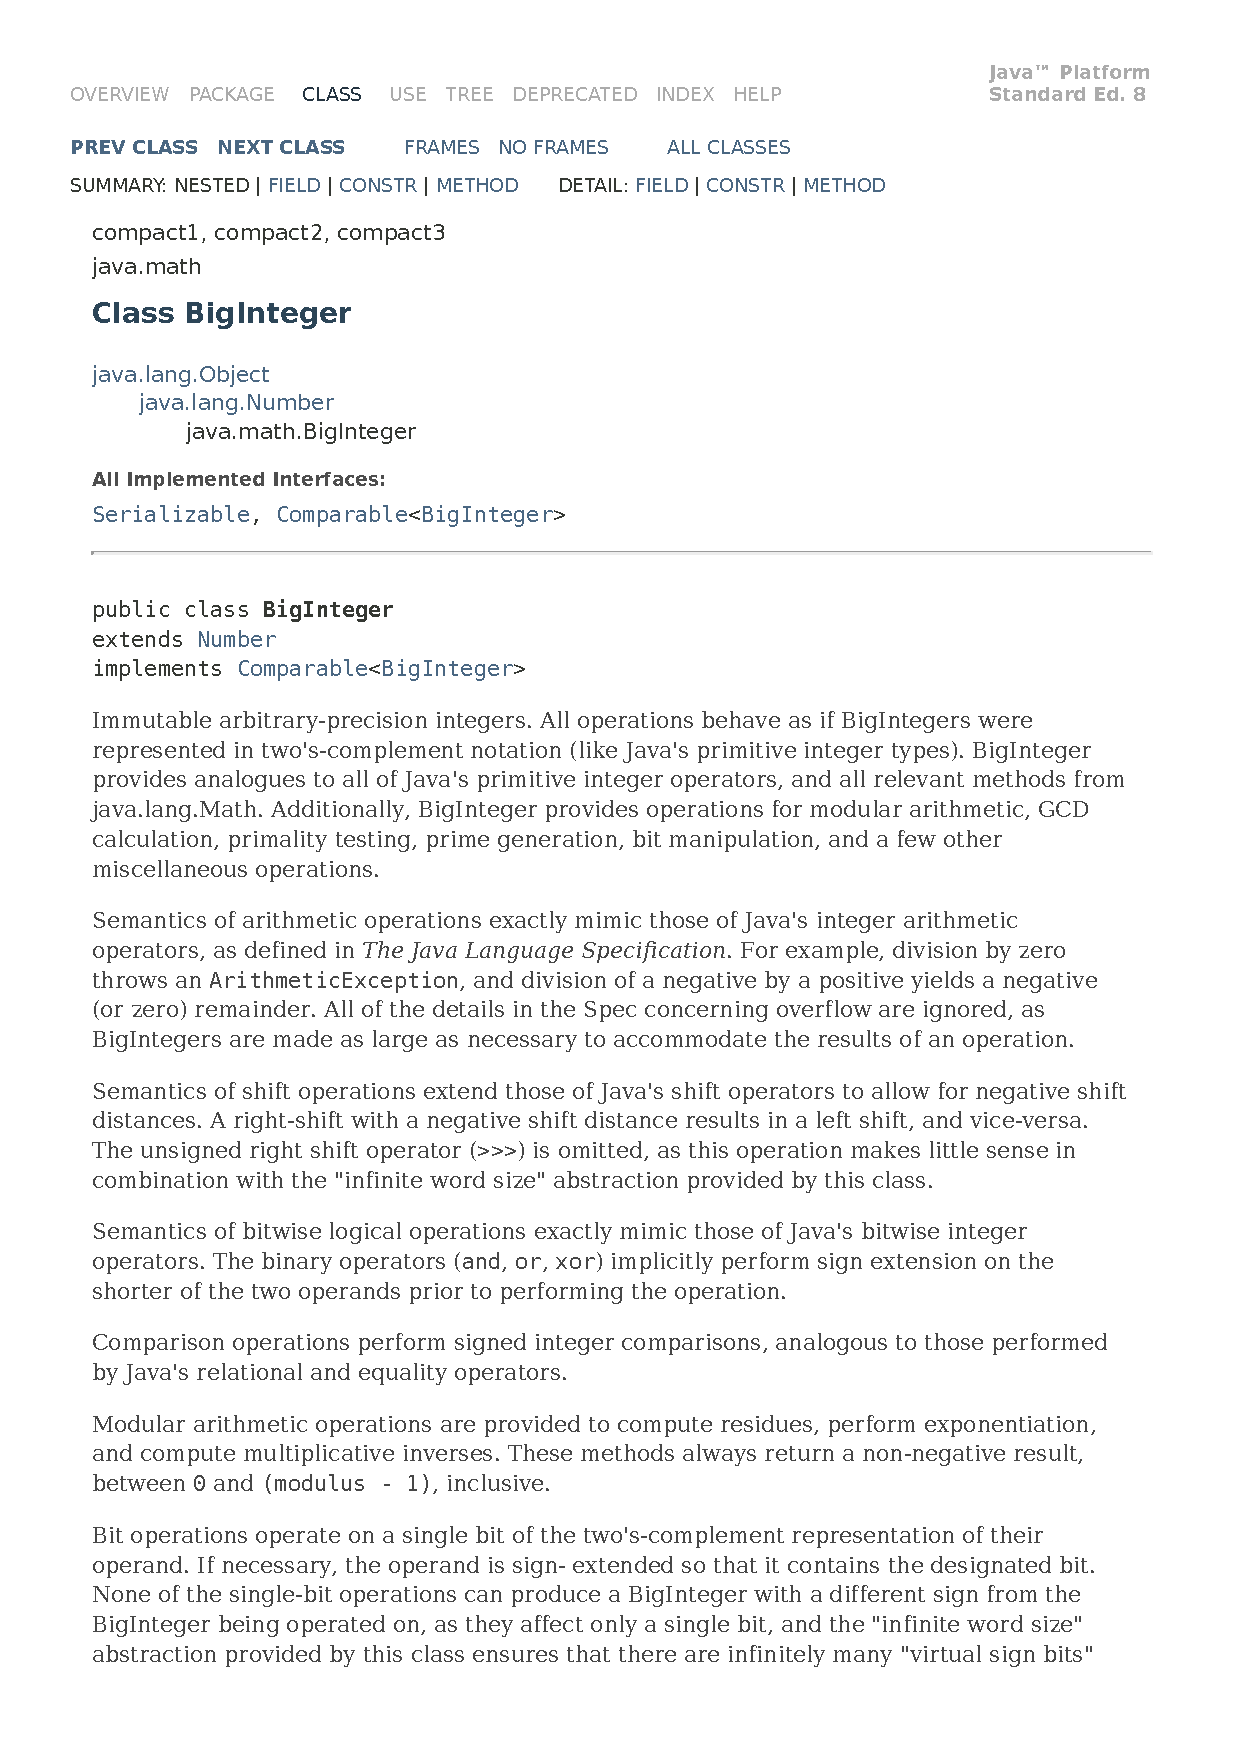
\includepdf[pages={1-6}]{source/biginteger.pdf}
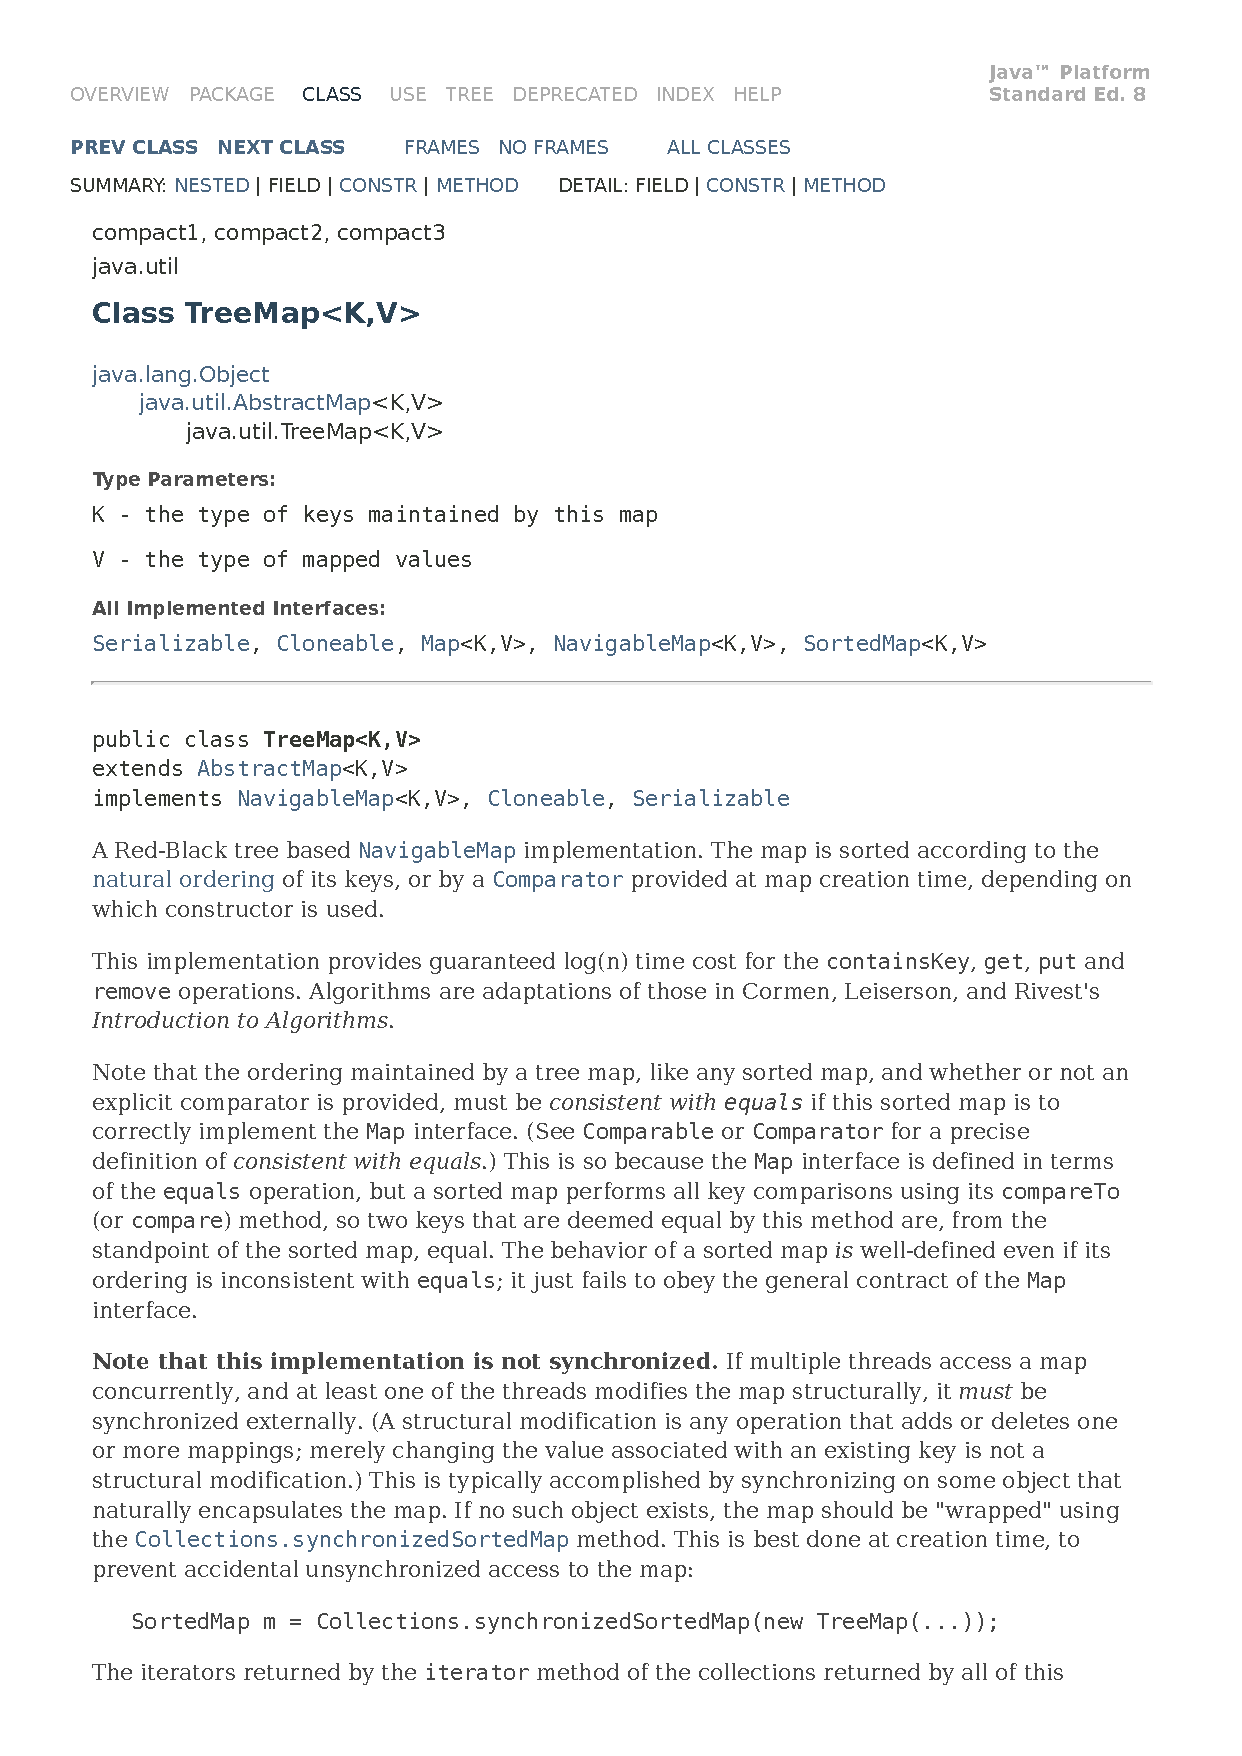
\includepdf[pages={1-5}]{source/treemap.pdf}

\section{gedit}

\javacode{gedit.ini}

%\subsection{BigInteger}

%\subsection{BigDecimal}

\section{数学}

%\subsection{常用积分表}

\subsection{常用数学公式}

\subsubsection{求和公式}

\begin{enumerate}
	\item $\sum_{k=1}^{n}(2k-1)^2 = \frac{n(4n^2-1)}{3}	$
	\item $\sum_{k=1}^{n}k^3 = [\frac{n(n+1)}{2}]^2	$
	\item $\sum_{k=1}^{n}(2k-1)^3 = n^2(2n^2-1)	$
	\item $\sum_{k=1}^{n}k^4 = \frac{n(n+1)(2n+1)(3n^2+3n-1)}{30}  $
	\item $\sum_{k=1}^{n}k^5 = \frac{n^2(n+1)^2(2n^2+2n-1)}{12}	$
	\item $\sum_{k=1}^{n}k(k+1) = \frac{n(n+1)(n+2)}{3}	$
	\item $\sum_{k=1}^{n}k(k+1)(k+2) = \frac{n(n+1)(n+2)(n+3)}{4} $
	\item $\sum_{k=1}^{n}k(k+1)(k+2)(k+3) = \frac{n(n+1)(n+2)(n+3)(n+4)}{5} $
\end{enumerate}

\subsubsection{斐波那契数列}

\begin{enumerate}
	\item $fib_0=0, fib_1=1, fib_n=fib_{n-1}+fib_{n-2}$
	\item $fib_{n+2} \cdot fib_n-fib_{n+1}^2=(-1)^{n+1}$
	\item $fib_{-n}=(-1)^{n-1}fib_n$
	\item $fib_{n+k}=fib_k \cdot fib_{n+1}+fib_{k-1} \cdot fib_n$
	\item $gcd(fib_m, fib_n)=fib_{gcd(m, n)}$
	\item $fib_m|fib_n^2\Leftrightarrow nfib_n|m$
\end{enumerate}

\subsubsection{错排公式}

\begin{enumerate}
	\item $D_n = (n-1)(D_{n-2}-D_{n-1})$
	\item $D_n = n! \cdot (1-\frac{1}{1!}+\frac{1}{2!}-\frac{1}{3!}+\ldots+\frac{(-1)^n}{n!})$
\end{enumerate}

\subsubsection{莫比乌斯函数}

$$\mu(n) = \begin{cases}
1 & \text{若}n=1\\
(-1)^k & \text{若}n\text{无平方数因子,且}n = p_1p_2\dots p_k\\
0 & \text{若}n\text{有大于}1\text{的平方数因数}
\end{cases}$$
$$\sum_{d|n}{\mu(d)} = \begin{cases}
1 & \text{若}n=1\\
0 & \text{其他情况}
\end{cases}$$
$$g(n) = \sum_{d|n}{f(d)} \Leftrightarrow f(n) = \sum_{d|n}{\mu(d)g(\frac{n}{d})}$$
$$g(x) = \sum_{n=1}^{[x]}f(\frac{x}{n}) \Leftrightarrow f(x) = \sum_{n=1}^{[x]}{\mu(n)g(\frac{x}{n})}$$

\subsubsection{伯恩赛德引理}
设$G$是一个有限群,作用在集合$X$上。对每个$g$属于$G$,令$X^g$表示$X$中在$g$作用下的不动元素,轨道数(记作$|X/G|$)由如下公式给出:
$$|X/G| = \frac{1}{|G|}\sum_{g \in G}|X^g|.\,$$

\subsubsection{五边形数定理}

设$p(n)$是$n$的拆分数,有$$p(n) = \sum_{k \in \mathbb{Z} \setminus \{0\}} (-1)^{k - 1} p\left(n - \frac{k(3k - 1)}{2}\right)$$

\subsubsection{树的计数}

\begin{enumerate}
	\item 有根树计数:$n+1$个结点的有根树的个数为
	$$a_{n+1} = \frac{\sum_{j=1}^{n}{j \cdot a_j \cdot{S_{n, j}}}}{n}$$
	其中,
	$$S_{n, j} = \sum_{i=1}^{n/j}{a_{n+1-ij}} = S_{n-j, j} + a_{n+1-j}$$
	\item 无根树计数:当$n$为奇数时,$n$个结点的无根树的个数为
	$$a_n-\sum_{i=1}^{n/2}{a_ia_{n-i}}$$
	当$n$为偶数时,$n$个结点的无根树的个数为
	$$a_n-\sum_{i=1}^{n/2}{a_ia_{n-i}}+\frac{1}{2}a_{\frac{n}{2}}(a_{\frac{n}{2}}+1)$$
	\item $n$个结点的完全图的生成树个数为
	$$n^{n-2}$$
	\item 矩阵-树定理:图$G$由$n$个结点构成,设$\bm{A}[G]$为图$G$的邻接矩阵、$\bm{D}[G]$为图$G$的度数矩阵,则图$G$的不同生成树的个数为$\bm{C}[G] = \bm{D}[G] - \bm{A}[G]$的任意一个$n-1$阶主子式的行列式值。
\end{enumerate}

\subsubsection{欧拉公式}

平面图的顶点个数、边数和面的个数有如下关系:
$$V - E + F = C+ 1$$
\indent 其中,$V$是顶点的数目,$E$是边的数目,$F$是面的数目,$C$是组成图形的连通部分的数目。当图是单连通图的时候,公式简化为:
$$V - E + F = 2$$

\subsubsection{皮克定理}

给定顶点坐标均是整点(或正方形格点)的简单多边形,其面积$A$和内部格点数目$i$、边上格点数目$b$的关系:
$$A = i + \frac{b}{2} - 1$$

\subsubsection{牛顿恒等式}

设$$\prod_{i = 1}^n{(x - x_i)} = a_n + a_{n - 1} x + \dots + a_1 x^{n - 1} + a_0 x^n$$
$$p_k = \sum_{i = 1}^n{x_i^k}$$
则$$a_0 p_k + a_1 p_{k - 1} + \cdots + a_{k - 1} p_1 + k a_k = 0$$

特别地,对于$$|\bm{A} - \lambda \bm{E}| = (-1)^n(a_n + a_{n - 1} \lambda + \cdots + a_1 \lambda^{n - 1} + a_0 \lambda^n)$$
有$$p_k = Tr(\bm{A}^k)$$

%\subsection{数论公式}

\subsection{平面几何公式}

\subsubsection{三角形}

\begin{enumerate}
	\item 半周长
	$$p=\frac{a+b+c}{2}$$
	\item 面积
	$$S=\frac{a \cdot H_a}{2}=\frac{ab \cdot sinC}{2}=\sqrt{p(p-a)(p-b)(p-c)}$$
	\item 中线
	$$M_a=\frac{\sqrt{2(b^2+c^2)-a^2}}{2}=\frac{\sqrt{b^2+c^2+2bc \cdot cosA}}{2}$$
	\item 角平分线 
	$$T_a=\frac{\sqrt{bc \cdot [(b+c)^2-a^2]}}{b+c}=\frac{2bc}{b+c}cos\frac{A}{2}$$
	\item 高线
	$$H_a=bsinC=csinB=\sqrt{b^2-(\frac{a^2+b^2-c^2}{2a})^2}$$
	\item 内切圆半径
	\begin{align*}
	r&=\frac{S}{p}=\frac{arcsin\frac{B}{2} \cdot sin\frac{C}{2}}{sin\frac{B+C}{2}}=4R \cdot sin\frac{A}{2}sin\frac{B}{2}sin\frac{C}{2}\\
	&=\sqrt{\frac{(p-a)(p-b)(p-c)}{p}}=p \cdot tan\frac{A}{2}tan\frac{B}{2}tan\frac{C}{2}
	\end{align*}
	\item 外接圆半径
	$$R=\frac{abc}{4S}=\frac{a}{2sinA}=\frac{b}{2sinB}=\frac{c}{2sinC}$$
\end{enumerate}

\subsubsection{四边形}

$D_1, D_2$为对角线,$M$对角线中点连线,$A$为对角线夹角,$p$为半周长
\begin{enumerate}
	\item $a^2+b^2+c^2+d^2=D_1^2+D_2^2+4M^2$
	\item $S=\frac{1}{2}D_1D_2sinA$
	\item 对于圆内接四边形
	$$ac+bd=D_1D_2$$
	\item 对于圆内接四边形
	$$S=\sqrt{(p-a)(p-b)(p-c)(p-d)}$$
\end{enumerate}

\subsubsection{正$n$边形}

$R$为外接圆半径,$r$为内切圆半径
\begin{enumerate}
	\item 中心角
	$$A=\frac{2\pi}{n}$$
	\item 内角
	$$C=\frac{n-2}{n}\pi$$
	\item 边长
	$$a=2\sqrt{R^2-r^2}=2R \cdot sin\frac{A}{2}=2r \cdot tan\frac{A}{2}$$
	\item 面积
	$$S=\frac{nar}{2}=nr^2 \cdot tan\frac{A}{2}=\frac{nR^2}{2} \cdot sinA=\frac{na^2}{4 \cdot tan\frac{A}{2}}$$
\end{enumerate}

\subsubsection{圆}

\begin{enumerate}
	\item 弧长
	$$l=rA$$
	\item 弦长
	$$a=2\sqrt{2hr-h^2}=2r\cdot sin\frac{A}{2}$$
	\item 弓形高
	$$h=r-\sqrt{r^2-\frac{a^2}{4}}=r(1-cos\frac{A}{2})=\frac{1}{2} \cdot arctan\frac{A}{4}$$
	\item 扇形面积
	$$S_1=\frac{rl}{2}=\frac{r^2A}{2}$$
	\item 弓形面积
	$$S_2=\frac{rl-a(r-h)}{2}=\frac{r^2}{2}(A-sinA)$$
\end{enumerate}

\subsubsection{棱柱}

\begin{enumerate}
	\item 体积
	$$V=Ah$$
	$A$为底面积,$h$为高
	\item 侧面积
	$$S=lp$$
	$l$为棱长,$p$为直截面周长
	\item 全面积
	$$T=S+2A$$
\end{enumerate}

\subsubsection{棱锥}

\begin{enumerate}
	\item 体积
	$$V=Ah$$
	$A$为底面积,$h$为高
	\item 正棱锥侧面积
	$$S=lp$$
	$l$为棱长,$p$为直截面周长
	\item 正棱锥全面积
	$$T=S+2A$$
\end{enumerate}

\subsubsection{棱台}

\begin{enumerate}
	\item 体积
	$$V=(A_1+A_2+\sqrt{A_1A_2}) \cdot \frac{h}{3}$$
	$A_1,A_2$为上下底面积,$h$为高
	\item 正棱台侧面积
	$$S=\frac{p_1+p_2}{2}l$$
	$p_1,p_2$为上下底面周长,$l$为斜高
	\item 正棱台全面积
	$$T=S+A_1+A_2$$
\end{enumerate}

\subsubsection{圆柱}

\begin{enumerate}
	\item 侧面积
	$$S=2\pi rh$$
	\item 全面积
	$$T=2\pi r(h+r)$$
	\item 体积
	$$V=\pi r^2h$$
\end{enumerate}

\subsubsection{圆锥}

\begin{enumerate}
	\item 母线
	$$l=\sqrt{h^2+r^2}$$
	\item 侧面积
	$$S=\pi rl$$
	\item 全面积
	$$T=\pi r(l+r)$$
	\item 体积
	$$V=\frac{\pi}{3} r^2h$$
\end{enumerate}

\subsubsection{圆台}

\begin{enumerate}
	\item 母线
	$$l=\sqrt{h^2+(r_1-r_2)^2}$$
	\item 侧面积
	$$S=\pi(r_1+r_2)l$$
	\item 全面积
	$$T=\pi r_1(l+r_1)+\pi r_2(l+r_2)$$
	\item 体积
	$$V=\frac{\pi}{3}(r_1^2+r_2^2+r_1r_2)h$$
\end{enumerate}

\subsubsection{球}

\begin{enumerate}
	\item 全面积
	$$T=4\pi r^2$$
	\item 体积
	$$V=\frac{4}{3}\pi r^3$$
\end{enumerate}

\subsubsection{球台}

\begin{enumerate}
	\item 侧面积
	$$S=2\pi rh$$
	\item 全面积
	$$T=\pi(2rh+r_1^2+r_2^2)$$
	\item 体积
	$$V=\frac{\pi h[3(r_1^2+r_2^2)+h^2]}{6}$$
\end{enumerate}

\subsubsection{球扇形}

\begin{enumerate}
	\item 全面积
	$$T=\pi r(2h+r_0)$$
	$h$为球冠高,$r_0$为球冠底面半径
	\item 体积
	$$V=\frac{2}{3}\pi r^2h$$
\end{enumerate}

\subsection{积分表}
\begin{footnotesize}
\noindent
\mbox{\vbox to 11pt{  \hbox{$
\int \frac{1}{1+x^2}dx = \tan^{-1}x
$}  }}
\\

\mbox{\vbox to 11pt{  \hbox{$
\int \frac{1}{a^2+x^2}dx = \frac{1}{a}\tan^{-1}\frac{x}{a}
$}  }}
\\

\mbox{\vbox to 11pt{  \hbox{$
\int \frac{x}{a^2+x^2}dx = \frac{1}{2}\ln|a^2+x^2|
$}  }}
\\

\mbox{\vbox to 11pt{  \hbox{$
\int \frac{x^2}{a^2+x^2}dx = x-a\tan^{-1}\frac{x}{a}
$}  }}
\\

\mbox{\vbox to 11pt{  \hbox{$
\int\sqrt{x^2 \pm a^2} dx  = \frac{1}{2}x\sqrt{x^2\pm a^2} 
%\nonumber \\ 
\pm\frac{1}{2}a^2 \ln \left | x + \sqrt{x^2\pm a^2} \right | 
$}  }}
\\
\mbox{\vbox to 11pt{  \hbox{$
\int  \sqrt{a^2 - x^2} dx  = \frac{1}{2} x \sqrt{a^2-x^2} 
%\nonumber \\  
+\frac{1}{2}a^2\tan^{-1}\frac{x}{\sqrt{a^2-x^2}}
$}  }}
\\
\mbox{\vbox to 11pt{  \hbox{$
\int \frac{x^2}{\sqrt{x^2 \pm a^2}} dx  = \frac{1}{2}x\sqrt{x^2 \pm a^2}
%\nonumber \\  
\mp \frac{1}{2}a^2 \ln \left| x + \sqrt{x^2\pm a^2} \right | 
$}  }}
\\

\mbox{\vbox to 11pt{  \hbox{$
\int \frac{1}{\sqrt{x^2 \pm a^2}} dx = \ln \left | x + \sqrt{x^2 \pm a^2} \right | 
$}  }}
\\

\mbox{\vbox to 11pt{  \hbox{$
\int \frac{1}{\sqrt{a^2 - x^2}} dx = \sin^{-1}\frac{x}{a} 
$}  }}
\\

\mbox{\vbox to 11pt{  \hbox{$
\int \frac{x}{\sqrt{x^2\pm a^2}}dx = \sqrt{x^2 \pm a^2} 
$}  }}
\\

\mbox{\vbox to 11pt{  \hbox{$
\int \frac{x}{\sqrt{a^2-x^2}}dx = -\sqrt{a^2-x^2} 
$}  }}
\\
\mbox{\vbox to 11pt{  \hbox{$
\int  \sqrt{a x^2 + b x + c} dx = 
\frac{b+2ax}{4a}\sqrt{ax^2+bx+c}
\nonumber \\  
+
\frac{4ac-b^2}{8a^{3/2}}\ln \left| 2ax + b + 2\sqrt{a(ax^2+bx^+c)}\right |
$}  }}
\\
\mbox{\vbox to 11pt{  \hbox{$
\int x^n e^{ax}\hspace{1pt}\text{d}x = \dfrac{x^n e^{ax}}{a} - 
\dfrac{n}{a}\int x^{n-1}e^{ax}\hspace{1pt}\text{d}x
$}  }} 
\\
\mbox{\vbox to 11pt{  \hbox{$
\int \sin^2 ax dx = \frac{x}{2} - \frac{1} {4a} \sin{2ax}
$}  }}
\\
\mbox{\vbox to 11pt{  \hbox{$
\int \sin^3 ax dx = -\frac{3 \cos ax}{4a} + \frac{\cos 3ax} {12a} 
$}  }}
\\
\mbox{\vbox to 11pt{  \hbox{$
\int \cos^2 ax dx = \frac{x}{2}+\frac{ \sin 2ax}{4a} 
$}  }}
\\
\mbox{\vbox to 11pt{  \hbox{$
\int \cos^3 ax dx = \frac{3 \sin ax}{4a}+\frac{ \sin 3ax}{12a} 
$}  }}
\\
\mbox{\vbox to 11pt{  \hbox{$
\int \tan ax dx = -\frac{1}{a} \ln \cos ax 
$}  }}
\\
\mbox{\vbox to 11pt{  \hbox{$
\int \tan^2 ax dx = -x + \frac{1}{a} \tan ax 
$}  }}
\\
\mbox{\vbox to 11pt{  \hbox{$
\int x \cos ax dx = \frac{1}{a^2} \cos ax + \frac{x}{a} \sin ax 
$}  }}
\\
\mbox{\vbox to 11pt{  \hbox{$
\int x^2 \cos ax dx = \frac{2 x \cos ax }{a^2} + \frac{ a^2 x^2 - 2  }{a^3} \sin ax 
$}  }}
\\
\mbox{\vbox to 11pt{  \hbox{$
\int x \sin ax dx = -\frac{x \cos ax}{a} + \frac{\sin ax}{a^2} 
$}  }}
\\
\mbox{\vbox to 11pt{  \hbox{$
\int x^2 \sin ax dx =\frac{2-a^2x^2}{a^3}\cos ax +\frac{ 2 x \sin ax}{a^2} 
$}  }}
\end{footnotesize}


\subsection{立体几何公式}

\subsubsection{球面三角公式}

设$a, b, c$是边长,$A, B, C$是所对的二面角,
有余弦定理$$cos a = cos b \cdot cos c + sin b \cdot sin c \cdot cos A$$
正弦定理$$\frac{sin A}{sin a} = \frac{sin B}{sin b} = \frac{sin C}{sin c}$$
三角形面积是$A + B + C - \pi$

\subsubsection{四面体体积公式}

$U, V, W, u, v, w$是四面体的$6$条棱,$U, V, W$构成三角形,$(U, u), (V, v), (W, w)$互为对棱,
则$$V = \frac{\sqrt{(s - 2a)(s - 2b)(s - 2c)(s - 2d)}}{192 uvw}$$
其中$$\left\{\begin{array}{lll}
a & = & \sqrt{xYZ}, \\
b & = & \sqrt{yZX}, \\
c & = & \sqrt{zXY}, \\
d & = & \sqrt{xyz}, \\
s & = & a + b + c + d, \\ 
X & = & (w - U + v)(U + v + w), \\
x & = & (U - v + w)(v - w + U), \\
Y & = & (u - V + w)(V + w + u), \\
y & = & (V - w + u)(w - u + V), \\
Z & = & (v - W + u)(W + u + v), \\
z & = & (W - u + v)(u - v + W)
\end{array}\right.$$

%\subsection{常用数表}

%\subsubsection{梅森数}

\subsection{博弈游戏}
\subsection*{巴什博奕}
	\begin{enumerate}
		\item
			只有一堆n个物品,两个人轮流从这堆物品中取物,规定每次至少取一个,最多取m个。最后取光者得胜。
		\item
			显然,如果$n=m+1$,那么由于一次最多只能取$m$个,所以,无论先取者拿走多少个,
			后取者都能够一次拿走剩余的物品,后者取胜。因此我们发现了如何取胜的法则:如果
			$n=(m+1)r+s$,(r为任意自然数,$s \leq m$),那么先取者要拿走$s$个物品,
			如果后取者拿走$k(k \leq m)$个,那么先取者再拿走$m+1-k$个,结果剩下$(m+1)(r-1)$
			个,以后保持这样的取法,那么先取者肯定获胜。总之,要保持给对手留下$(m+1)$的倍数,
			就能最后获胜。
	\end{enumerate}
\subsection*{威佐夫博弈}
	\begin{enumerate}
		\item
			有两堆各若干个物品,两个人轮流从某一堆或同时从两堆中取同样多的物品,规定每次至少取
			一个,多者不限,最后取光者得胜。
		\item
			判断一个局势$(a, b)$为奇异局势(必败态)的方法:$\displaystyle a_k =[k (1+\sqrt{5})/2],b_k= a_k + k$
	\end{enumerate}
\subsection*{阶梯博奕}
	\begin{enumerate}
		\item
			博弈在一列阶梯上进行,每个阶梯上放着自然数个点,两个人进行阶梯博弈,
			每一步则是将一个阶梯上的若干个点(至少一个)移到前面去,最后没有点
			可以移动的人输。
		\item
			解决方法:把所有奇数阶梯看成N堆石子,做NIM。(把石子从奇数堆移动到偶数
			堆可以理解为拿走石子,就相当于几个奇数堆的石子在做Nim)
	\end{enumerate}
\subsection*{图上删边游戏}
	\subsubsection*{链的删边游戏}
		\begin{enumerate}
			\item
				游戏规则:对于一条链,其中一个端点是根,两人轮流删边,脱离根的部分也算被删去,最后没边可删的人输。
			\item
				做法:$sg[i] = n - dist(i) - 1$(其中$n$表示总点数,$dist(i)$表示离根的距离)
		\end{enumerate}
	\subsubsection*{树的删边游戏}
		\begin{enumerate}
			\item
				游戏规则:对于一棵有根树,两人轮流删边,脱离根的部分也算被删去,没边可删的人输。
			\item
				做法:叶子结点的$sg=0$,其他节点的$sg$等于儿子结点的$sg+1$的异或和。
		\end{enumerate}
	\subsubsection*{局部连通图的删边游戏}
		\begin{enumerate}
			\item
				游戏规则:在一个局部连通图上,两人轮流删边,脱离根的部分也算被删去,没边可删的人输。
				局部连通图的构图规则是,在一棵基础树上加边得到,所有形成的环保证不共用边,且只与基础树有一个公共点。
			\item
				做法:去掉所有的偶环,将所有的奇环变为长度为1的链,然后做树的删边游戏。
		\end{enumerate}

\subsection{常用数学公式}
\subsection{求和公式}
	\begin{enumerate}
		\item $\sum_{k=1}^{n}(2k-1)^2 = \frac{n(4n^2-1)}{3}	$
		\item $\sum_{k=1}^{n}k^3 = [\frac{n(n+1)}{2}]^2	$
		\item $\sum_{k=1}^{n}(2k-1)^3 = n^2(2n^2-1)	$
		\item $\sum_{k=1}^{n}k^4 = \frac{n(n+1)(2n+1)(3n^2+3n-1)}{30}  $
		\item $\sum_{k=1}^{n}k^5 = \frac{n^2(n+1)^2(2n^2+2n-1)}{12}	$
		\item $\sum_{k=1}^{n}k(k+1) = \frac{n(n+1)(n+2)}{3}	$
		\item $\sum_{k=1}^{n}k(k+1)(k+2) = \frac{n(n+1)(n+2)(n+3)}{4} $
		\item $\sum_{k=1}^{n}k(k+1)(k+2)(k+3) = \frac{n(n+1)(n+2)(n+3)(n+4)}{5} $
	\end{enumerate}
\subsection{斐波那契数列}
	\begin{enumerate}
		\item $fib_0=0, fib_1=1, fib_n=fib_{n-1}+fib_{n-2}$
		\item $fib_{n+2} \cdot fib_n-fib_{n+1}^2=(-1)^{n+1}$
		\item $fib_{-n}=(-1)^{n-1}fib_n$
		\item $fib_{n+k}=fib_k \cdot fib_{n+1}+fib_{k-1} \cdot fib_n$
		\item $gcd(fib_m, fib_n)=fib_{gcd(m, n)}$
		\item $fib_m|fib_n^2\Leftrightarrow nfib_n|m$
	\end{enumerate}
\subsection{错排公式}
	\begin{enumerate}
		\item $D_n = (n-1)(D_{n-2}-D_{n-1})$
		\item $D_n = n! \cdot (1-\frac{1}{1!}+\frac{1}{2!}-\frac{1}{3!}+\ldots+\frac{(-1)^n}{n!})$
	\end{enumerate}
\subsection{莫比乌斯函数}
	$$\mu(n) = \begin{cases}
		1 & \text{若}n=1\\
		(-1)^k & \text{若}n\text{无平方数因子,且}n = p_1p_2\dots p_k\\
		0 & \text{若}n\text{有大于}1\text{的平方数因数}
	\end{cases}$$
	$$\sum_{d|n}{\mu(d)} = \begin{cases}
		1 & \text{若}n=1\\
		0 & \text{其他情况}
	\end{cases}$$
	$$g(n) = \sum_{d|n}{f(d)} \Leftrightarrow f(n) = \sum_{d|n}{\mu(d)g(\frac{n}{d})}$$
	$$g(x) = \sum_{n=1}^{[x]}f(\frac{x}{n}) \Leftrightarrow f(x) = \sum_{n=1}^{[x]}{\mu(n)g(\frac{x}{n})}$$
\subsection{Burnside引理}
	设$G$是一个有限群,作用在集合$X$上。对每个$g$属于$G$,令$X^g$表示$X$中在$g$作用下的不动元素,轨道数(记作$|X/G|$)由如下公式给出:
		$$|X/G| = \frac{1}{|G|}\sum_{g \in G}|X^g|.\,$$
\subsection{五边形数定理}
	设$p(n)$是$n$的拆分数,有$$p(n) = \sum_{k \in \mathbb{Z} \setminus \{0\}} (-1)^{k - 1} p\left(n - \frac{k(3k - 1)}{2}\right)$$
\subsection{树的计数}
	\begin{enumerate}
		\item 有根树计数:$n+1$个结点的有根树的个数为
			$$a_{n+1} = \frac{\sum_{j=1}^{n}{j \cdot a_j \cdot{S_{n, j}}}}{n}$$
		其中,
			$$S_{n, j} = \sum_{i=1}^{n/j}{a_{n+1-ij}} = S_{n-j, j} + a_{n+1-j}$$
		\item 无根树计数:当$n$为奇数时,$n$个结点的无根树的个数为
			$$a_n-\sum_{i=1}^{n/2}{a_ia_{n-i}}$$
		当$n$为偶数时,$n$个结点的无根树的个数为
			$$a_n-\sum_{i=1}^{n/2}{a_ia_{n-i}}+\frac{1}{2}a_{\frac{n}{2}}(a_{\frac{n}{2}}+1)$$
		\item $n$个结点的完全图的生成树个数为
			$$n^{n-2}$$
		\item 矩阵-树定理:
		图$G$由$n$个结点构成,设$\bm{A}[G]$为图$G$的邻接矩阵、$\bm{D}[G]$为图$G$的度数矩阵,
		则图$G$的不同生成树的个数为$\bm{C}[G] = \bm{D}[G] - \bm{A}[G]$的任意一个$n-1$阶主子式的行列式值。
	\end{enumerate}
\subsection{欧拉公式}
	平面图的顶点个数、边数和面的个数有如下关系:
		$$V - E + F = C+ 1$$
	\indent 其中,$V$是顶点的数目,$E$是边的数目,$F$是面的数目,$C$是组成图形的连通部分的数目。当图是单连通图的时候,公式简化为:
		$$V - E + F = 2$$
\subsection{皮克定理}
	给定顶点坐标均是整点(或正方形格点)的简单多边形,其面积$A$和内部格点数目$i$、边上格点数目$b$的关系:
		$$A = i + \frac{b}{2} - 1$$
\subsection{牛顿恒等式}
	设$$\prod_{i = 1}^n{(x - x_i)} = a_n + a_{n - 1} x + \dots + a_1 x^{n - 1} + a_0 x^n$$
	$$p_k = \sum_{i = 1}^n{x_i^k}$$
	则$$a_0 p_k + a_1 p_{k - 1} + \cdots + a_{k - 1} p_1 + k a_k = 0$$\par
	特别地,对于$$|\bm{A} - \lambda \bm{E}| = (-1)^n(a_n + a_{n - 1} \lambda + \cdots + a_1 \lambda^{n - 1} + a_0 \lambda^n)$$
	有$$p_k = \mathrm{Tr}(\bm{A}^k)$$
%\section{数论公式}
\section{平面几何公式}
\subsection{三角形}
	\begin{enumerate}
		\item 半周长
			$$p=\frac{a+b+c}{2}$$
		\item 面积
			$$S=\frac{a \cdot H_a}{2}=\frac{ab \cdot sinC}{2}=\sqrt{p(p-a)(p-b)(p-c)}$$
		\item 中线
			$$M_a=\frac{\sqrt{2(b^2+c^2)-a^2}}{2}=\frac{\sqrt{b^2+c^2+2bc \cdot cosA}}{2}$$
		\item 角平分线 
			$$T_a=\frac{\sqrt{bc \cdot [(b+c)^2-a^2]}}{b+c}=\frac{2bc}{b+c}cos\frac{A}{2}$$
		\item 高线
			$$H_a=bsinC=csinB=\sqrt{b^2-(\frac{a^2+b^2-c^2}{2a})^2}$$
		\item 内切圆半径
			\begin{align*}
				r&=\frac{S}{p}=\frac{arcsin\frac{B}{2} \cdot sin\frac{C}{2}}{sin\frac{B+C}{2}}=4R \cdot sin\frac{A}{2}sin\frac{B}{2}sin\frac{C}{2}\\
				&=\sqrt{\frac{(p-a)(p-b)(p-c)}{p}}=p \cdot tan\frac{A}{2}tan\frac{B}{2}tan\frac{C}{2}
			\end{align*}
		\item 外接圆半径
			$$R=\frac{abc}{4S}=\frac{a}{2sinA}=\frac{b}{2sinB}=\frac{c}{2sinC}$$
	\end{enumerate}
\subsection{四边形}
	$D_1, D_2$为对角线,$M$对角线中点连线,$A$为对角线夹角,$p$为半周长
	\begin{enumerate}
		\item $a^2+b^2+c^2+d^2=D_1^2+D_2^2+4M^2$
		\item $S=\frac{1}{2}D_1D_2sinA$
		\item 对于圆内接四边形
			$$ac+bd=D_1D_2$$
		\item 对于圆内接四边形
			$$S=\sqrt{(p-a)(p-b)(p-c)(p-d)}$$
	\end{enumerate}
\subsection{正$n$边形}
	$R$为外接圆半径,$r$为内切圆半径
	\begin{enumerate}
		\item 中心角
			$$A=\frac{2\pi}{n}$$
		\item 内角
			$$C=\frac{n-2}{n}\pi$$
		\item 边长
			$$a=2\sqrt{R^2-r^2}=2R \cdot sin\frac{A}{2}=2r \cdot tan\frac{A}{2}$$
		\item 面积
			$$S=\frac{nar}{2}=nr^2 \cdot tan\frac{A}{2}=\frac{nR^2}{2} \cdot sinA=\frac{na^2}{4 \cdot tan\frac{A}{2}}$$
	\end{enumerate}
\subsection{圆}
	\begin{enumerate}
		\item 弧长
			$$l=rA$$
		\item 弦长
			$$a=2\sqrt{2hr-h^2}=2r\cdot sin\frac{A}{2}$$
		\item 弓形高
			$$h=r-\sqrt{r^2-\frac{a^2}{4}}=r(1-cos\frac{A}{2})=\frac{1}{2} \cdot arctan\frac{A}{4}$$
		\item 扇形面积
			$$S_1=\frac{rl}{2}=\frac{r^2A}{2}$$
		\item 弓形面积
			$$S_2=\frac{rl-a(r-h)}{2}=\frac{r^2}{2}(A-sinA)$$
	\end{enumerate}
\subsection{棱柱}
	\begin{enumerate}
		\item 体积
			$$V=Ah$$
			$A$为底面积,$h$为高
		\item 侧面积
			$$S=lp$$
			$l$为棱长,$p$为直截面周长
		\item 全面积
			$$T=S+2A$$
	\end{enumerate}
\subsection{棱锥}
	\begin{enumerate}
		\item 体积
			$$V=Ah$$
			$A$为底面积,$h$为高
		\item 正棱锥侧面积
			$$S=lp$$
			$l$为棱长,$p$为直截面周长
		\item 正棱锥全面积
			$$T=S+2A$$
	\end{enumerate}
\subsection{棱台}
	\begin{enumerate}
		\item 体积
			$$V=(A_1+A_2+\sqrt{A_1A_2}) \cdot \frac{h}{3}$$
			$A_1,A_2$为上下底面积,$h$为高
		\item 正棱台侧面积
			$$S=\frac{p_1+p_2}{2}l$$
			$p_1,p_2$为上下底面周长,$l$为斜高
		\item 正棱台全面积
			$$T=S+A_1+A_2$$
	\end{enumerate}
\subsection{圆柱}
	\begin{enumerate}
		\item 侧面积
			$$S=2\pi rh$$
		\item 全面积
			$$T=2\pi r(h+r)$$
		\item 体积
			$$V=\pi r^2h$$
	\end{enumerate}
\subsection{圆锥}
	\begin{enumerate}
		\item 母线
			$$l=\sqrt{h^2+r^2}$$
		\item 侧面积
			$$S=\pi rl$$
		\item 全面积
			$$T=\pi r(l+r)$$
		\item 体积
			$$V=\frac{\pi}{3} r^2h$$
	\end{enumerate}
\subsection{圆台}
	\begin{enumerate}
		\item 母线
			$$l=\sqrt{h^2+(r_1-r_2)^2}$$
		\item 侧面积
			$$S=\pi(r_1+r_2)l$$
		\item 全面积
			$$T=\pi r_1(l+r_1)+\pi r_2(l+r_2)$$
		\item 体积
			$$V=\frac{\pi}{3}(r_1^2+r_2^2+r_1r_2)h$$
	\end{enumerate}
\subsection{球}
	\begin{enumerate}
		\item 全面积
			$$T=4\pi r^2$$
		\item 体积
			$$V=\frac{4}{3}\pi r^3$$
	\end{enumerate}
\subsection{球台}
	\begin{enumerate}
		\item 侧面积
			$$S=2\pi rh$$
		\item 全面积
			$$T=\pi(2rh+r_1^2+r_2^2)$$
		\item 体积
			$$V=\frac{\pi h[3(r_1^2+r_2^2)+h^2]}{6}$$
	\end{enumerate}
\subsection{球扇形}
	\begin{enumerate}
		\item 全面积
			$$T=\pi r(2h+r_0)$$
			$h$为球冠高,$r_0$为球冠底面半径
		\item 体积
			$$V=\frac{2}{3}\pi r^2h$$
	\end{enumerate}
\section{立体几何公式}
\subsection{球面三角公式}
	设$a, b, c$是边长,$A, B, C$是所对的二面角,
	有余弦定理$$cos a = cos b \cdot cos c + sin b \cdot sin c \cdot cos A$$
	正弦定理$$\frac{sin A}{sin a} = \frac{sin B}{sin b} = \frac{sin C}{sin c}$$
	三角形面积是$A + B + C - \pi$
\subsection{四面体体积公式}
	$U, V, W, u, v, w$是四面体的$6$条棱,$U, V, W$构成三角形,$(U, u), (V, v), (W, w)$互为对棱,
	则$$V = \frac{\sqrt{(s - 2a)(s - 2b)(s - 2c)(s - 2d)}}{192 uvw}$$
	其中$$\left\{\begin{array}{lll}
			a & = & \sqrt{xYZ}, \\
			b & = & \sqrt{yZX}, \\
			c & = & \sqrt{zXY}, \\
			d & = & \sqrt{xyz}, \\
			s & = & a + b + c + d, \\ 
			X & = & (w - U + v)(U + v + w), \\
			x & = & (U - v + w)(v - w + U), \\
			Y & = & (u - V + w)(V + w + u), \\
			y & = & (V - w + u)(w - u + V), \\
			Z & = & (v - W + u)(W + u + v), \\
			z & = & (W - u + v)(u - v + W)
		\end{array}\right.$$


\section{附录}
\subsection{NTT素数及原根列表}
\begin{spacing}{0.97}
\rowcolors{2}{black!25}{white}
\noindent \begin{tabular}{ccc}
\toprule
       Id & Primes & Primitive Root\\
\midrule 1 & 7340033 & 3\\
 2 & 13631489 & 15\\
 3 & 23068673 & 3\\
 4 & 26214401 & 3\\
 5 & 28311553 & 5\\
 6 & 69206017 & 5\\
 7 & 70254593 & 3\\
 8 & 81788929 & 7\\
 9 & 101711873 & 3\\
 10 & 104857601 & 3\\
 11 & 111149057 & 3\\
 12 & 113246209 & 7\\
 13 & 120586241 & 6\\
 14 & 132120577 & 5\\
 15 & 136314881 & 3\\
 16 & 138412033 & 5\\
 17 & 141557761 & 26\\
 18 & 147849217 & 5\\
 19 & 155189249 & 6\\
 20 & 158334977 & 3\\
 21 & 163577857 & 23\\
 22 & 167772161 & 3\\
 23 & 169869313 & 5\\
 24 & 185597953 & 5\\
 25 & 186646529 & 3\\
 26 & 199229441 & 3\\
 27 & 204472321 & 19\\
 28 & 211812353 & 3\\
 29 & 221249537 & 3\\
 30 & 230686721 & 6\\
 31 & 246415361 & 3\\
 32 & 249561089 & 3\\
 33 & 257949697 & 5\\
 34 & 270532609 & 22\\
 35 & 274726913 & 3\\
 36 & 290455553 & 3\\
 37 & 305135617 & 5\\
\bottomrule
\end{tabular}
\rowcolors{2}{black!25}{white}
\begin{tabular}{ccc}
\toprule
       Id & Primes & Primitive Root\\
 \midrule
 38 & 311427073 & 7\\
 39 & 330301441 & 22\\
 40 & 347078657 & 3\\
 41 & 359661569 & 3\\
 42 & 361758721 & 29\\
 43 & 377487361 & 7\\
 44 & 383778817 & 5\\
 45 & 387973121 & 6\\
 46 & 399507457 & 5\\
 47 & 409993217 & 3\\
 48 & 415236097 & 5\\
 49 & 447741953 & 3\\
 50 & 459276289 & 11\\
 51 & 463470593 & 3\\
 52 & 468713473 & 5\\
 53 & 469762049 & 3\\
 54 & 493879297 & 10\\
 55 & 531628033 & 5\\
 56 & 576716801 & 6\\
 57 & 581959681 & 11\\
 58 & 595591169 & 3\\
 59 & 597688321 & 11\\
 60 & 605028353 & 3\\
 61 & 635437057 & 11\\
 62 & 639631361 & 6\\
 63 & 645922817 & 3\\
 64 & 648019969 & 17\\
 65 & 655360001 & 3\\
 66 & 666894337 & 5\\
 67 & 683671553 & 3\\
 68 & 710934529 & 17\\
 69 & 715128833 & 3\\
 70 & 718274561 & 3\\
 71 & 740294657 & 3\\
 72 & 745537537 & 5\\
 73 & 754974721 & 11\\
 74 & 770703361 & 11\\
\bottomrule
\end{tabular}
\rowcolors{2}{black!25}{white}
\begin{tabular}{ccc}
\toprule
       Id & Primes & Primitive Root\\
 \midrule
 75 & 786432001 & 7\\
 76 & 799014913 & 13\\
 77 & 800063489 & 3\\
 78 & 802160641 & 11\\
 79 & 818937857 & 5\\
 80 & 824180737 & 5\\
 81 & 833617921 & 13\\
 82 & 850395137 & 3\\
 83 & 862978049 & 3\\
 84 & 880803841 & 26\\
 85 & 883949569 & 7\\
 86 & 897581057 & 3\\
 87 & 899678209 & 7\\
 88 & 907018241 & 3\\
 89 & 913309697 & 3\\
 90 & 918552577 & 5\\
 91 & 919601153 & 3\\
 92 & 924844033 & 5\\
 93 & 925892609 & 3\\
 94 & 935329793 & 3\\
 95 & 938475521 & 3\\
 96 & 940572673 & 7\\
 97 & 943718401 & 7\\
 98 & 950009857 & 7\\
 99 & 957349889 & 6\\
 100 & 962592769 & 7\\
 101 & 972029953 & 10\\
 102 & 975175681 & 17\\
 103 & 976224257 & 3\\
 104 & 985661441 & 3\\
 105 & 998244353 & 3\\
 106 & 1004535809 & 3\\
 107 & 1007681537 & 3\\
 108 & 1012924417 & 5\\
 109 & 1045430273 & 3\\
 110 & 1051721729 & 6\\
 111 & 1053818881 & 7\\
\bottomrule
\end{tabular}
\end{spacing}

\subsection{cheat.pdf}
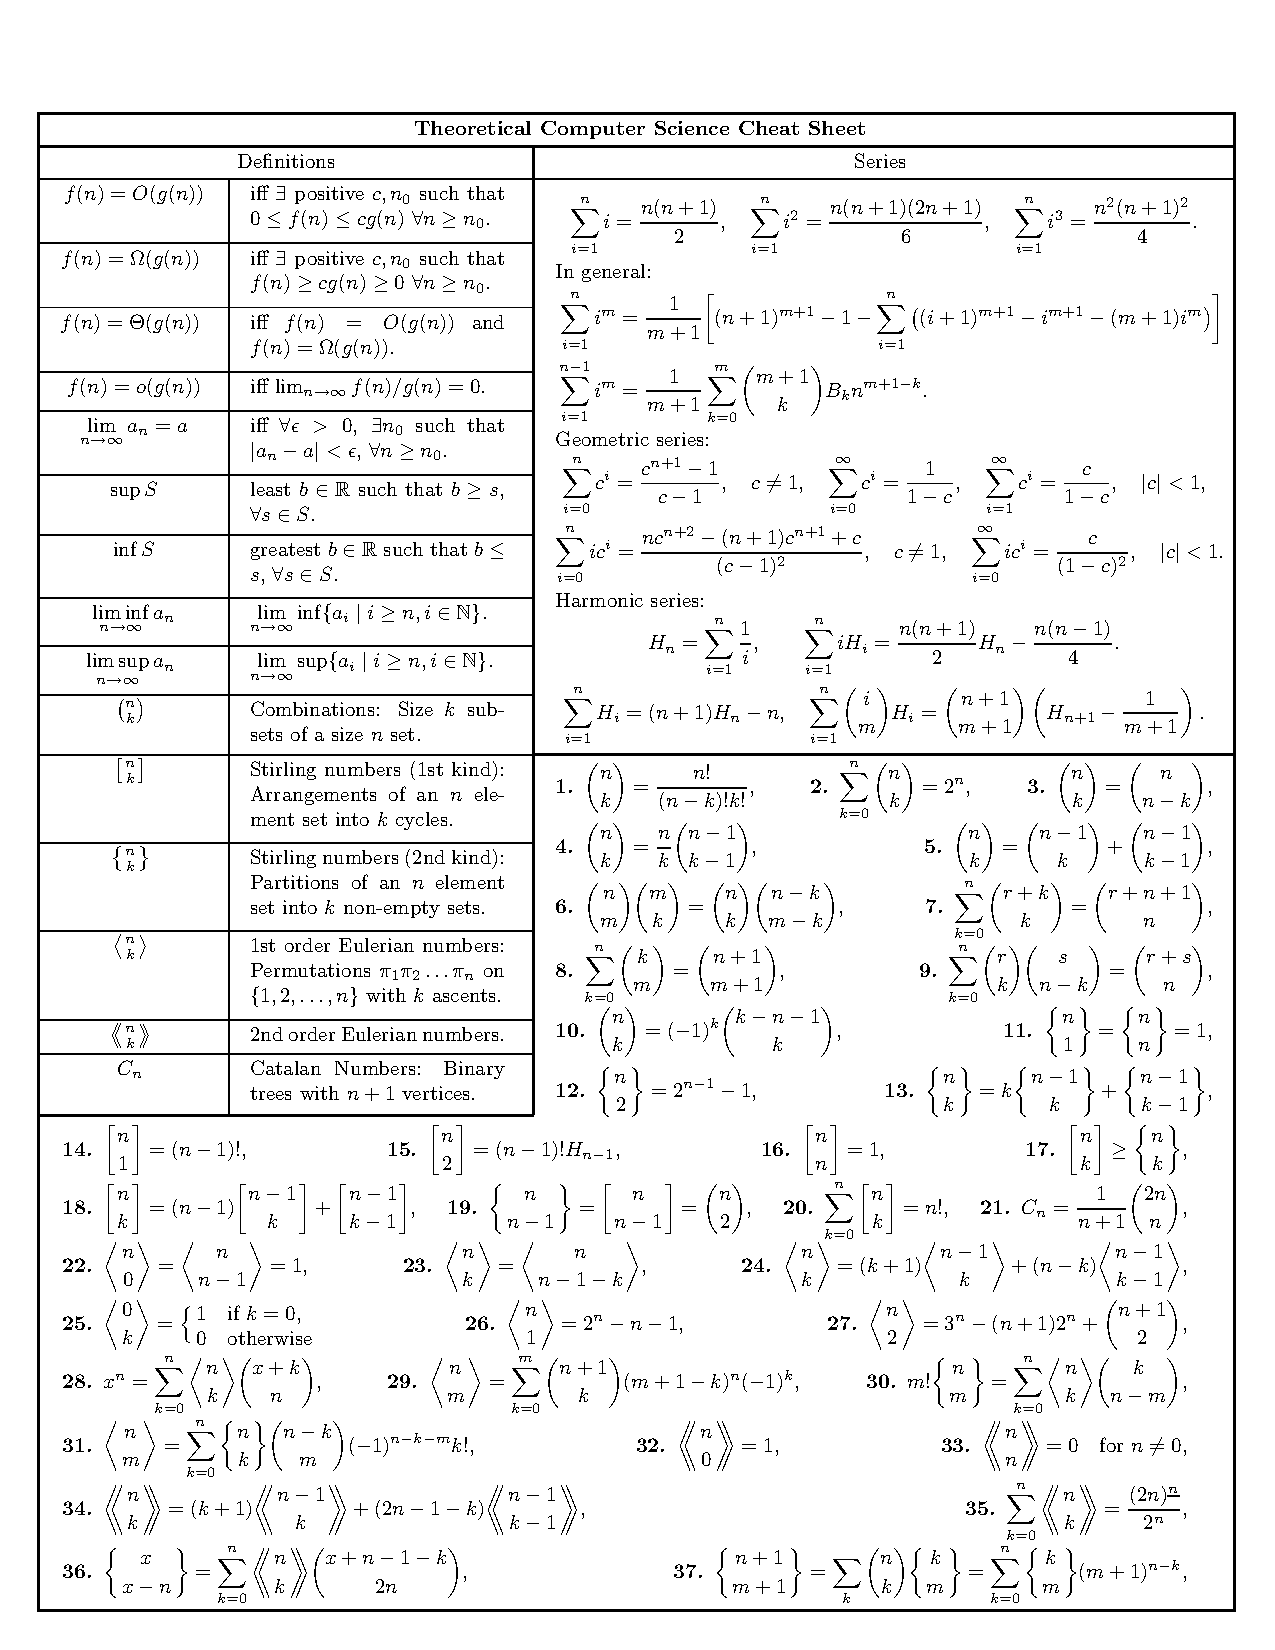
\includepdf[pages=-]{source/Appendix/cheat.pdf}

\end{document}
